\documentclass{article}
\usepackage[utf8]{inputenc}
\usepackage[hidelinks]{hyperref}
\usepackage{xcolor}
\usepackage[T1]{fontenc}
\usepackage{listings}
\usepackage{xcolor}
\usepackage{graphicx}
\usepackage[a4paper, left = 3cm, right = 3cm, top =2cm]{geometry}
\definecolor{codegreen}{rgb}{0,0.6,0}
\definecolor{codegray}{rgb}{0.5,0.5,0.5}
\definecolor{codepurple}{rgb}{0.58,0,0.82}
\definecolor{backcolour}{rgb}{0.95,0.95,0.92}
\definecolor{redflag}{rgb}{0.266,0,0}
\definecolor{blueflagg}{rgb}{0,87,214}
\definecolor{darkblueflag}{rgb}{0,33,66}
\definecolor{customGreen}{HTML}{228B22}
\lstdefinestyle{mystyle}{
    backgroundcolor=\color{backcolour},   
    commentstyle=\color{codegreen},
    keywordstyle=\color{magenta},
    numberstyle=\tiny\color{codegray},
    stringstyle=\color{codepurple},
    basicstyle=\ttfamily\footnotesize,
    breakatwhitespace=false,         
    breaklines=true,                 
    captionpos=b,                    
    keepspaces=true,                 
    numbers=left,                    
    numbersep=5pt,                  
    showspaces=false,                
    showstringspaces=false,
    showtabs=false,                  
    tabsize=2
}
\lstset{keepspaces=true, style=mystyle}

\begin{document}
\begin{titlepage}
    \begin{center}
    {
\includegraphics[width=0.15\textwidth]{img/matcom.jpg}\par}
    \vspace{0.1cm}
    {\bfseries\LARGE Ciencia de Datos \par}
    \vspace{0.2cm}
    {\scshape\Large  Facultad de Matamática y Computación\par}
    \vspace{0.6cm}
    {\scshape\Huge{{\textbf{Introducción a la Ciencia de Datos \\ Proyecto Final}} \par}
    \vspace{0.2cm}
    {\itshape\Large {\large{\textit{Procesos migratorios en Cienfuegos}}} \par}
    \vspace{0.8cm}
    {\large Autor: \\ \normalsize{Luis Ernesto Serras Rimada} \par}
    \vspace{0.5cm}
    {
\includegraphics[width=0.85\textwidth]{img/perla.png}}
    \end{center}
\end{titlepage}
\newpage
\section{Introducción}
La búsqueda de mejores oportunidades de empleo y educación es un impulso fundamental que motiva a las personas a migrar, tanto a nivel interno como externo. Este fenómeno refleja no solo la aspiración individual de alcanzar una vida más digna y satisfactoria, sino también un contexto socioeconómico que, en muchos casos, limita el desarrollo personal y profesional en sus lugares de origen. La decisión de emprender este camino, aunque a menudo dolorosa y compleja, simboliza la lucha por la superación y el deseo de construir un futuro mejor. Al mismo tiempo, pone de manifiesto las disparidades entre regiones, donde lugares como La Habana ofrecen un abanico más amplio de oportunidades comparado con provincias como \textcolor{blue}{Cienfuegos}. En última instancia, este deseo de progreso se convierte en una fuerza dinámica que puede transformar realidades, tanto para los individuos como para las comunidades a las que pertenecen.


\section{Desarrollo}
\subsection{Recopilación y procesamiento de los datos}
La fuente principal de los datos manejados fueron las series estadísticas y anuarios de la \textcolor{blue}{Oficina Nacional de Estadosisticas e Información (ONEI)}. Las series estadísticas empleadas en formato .xls (llevados a formato csv) fueron reacomodados a mano mayormente para luego limpiarlos haciendo uso del modulo \textcolor{green}{csv} de \textcolor{blue}{Python}.\\ 
El análisis en su totalidad fue realizado manejando datos procesados y cargados unicamente desde la manipulación directa de los \textcolor{green}{csv} por medio del módulo de \textcolor{blue}{pandas}.

\begin{lstlisting}[language=Python, caption=Funcion para la limpieza de los csv (eliminar espacios adicionales)]
# Function to skip initial space on csv's files
def skipinitalspace_csv(path:str):
    from csv import reader, writer
    data = []
    with open(path, "r") as f:
        reader = reader(f, skipinitialspace=True)
        for i in reader:
            data.append(i)
    with open(path, 'w') as f:
        writer = writer(f)
        writer.writerows(data)
\end{lstlisting}


\begin{lstlisting}[language=Python, caption=Funcion utilizada para parte del procesamiento de algunos datos]
    def migratory_movements(df: pd.core.frame.DataFrame, type:str="prov") -> list[pd.core.frame.DataFrame]:
    #Funcion para el procesamiento de los datos
    if type == "prov":
        year2012, year2013, year2014, year2015, year2016, year2017, year2018, year2019, year2020, year2021, year2022 = 0,0,0,0,0,0,0,0,0,0,0
        dfs = [year2012, year2013, year2014, year2015, year2016, year2017, year2018, year2019, year2020, year2021, year2022]
        i = 1
        for index in range(len(dfs)):
            j = i + 49
            dfs[index] = df.iloc[i:j:3,:]
            dfs[index].set_index("PROCEDENCIA/DESTINO", inplace=True)
            dfs[index].index.name='Anno'
            i = j + 3
    elif type == "mun":
        year2019, year2020, year2021, year2022 = 0,0,0,0
        dfs = [year2019, year2020, year2021, year2022]
        i = 1
        for index in range(len(dfs)):
            j = i + 8
            dfs[index] = df.iloc[i:j,:]
            dfs[index].set_index("ANNOS", inplace=True)
            dfs[index].index.name='Anno'
            i = j + 1
    elif type == "etc":
        prov1, prov2, prov3, prov4, prov5, prov6, prov7, prov8, prov9, prov10, prov11, prov12, prov13, prov14, prov15 = 0,0,0,0,0,0,0,0,0,0,0,0,0,0,0
        dfs = [prov1, prov2, prov3, prov4, prov5, prov6, prov7, prov8, prov9, prov10, prov11, prov12, prov13, prov14, prov15]
        i = 1
        for index in range(len(dfs)):
            j = i + 12
            dfs[index] = df.iloc[i:j,:]
            dfs[index].set_index("PROVINCIAS/ANNOS", inplace=True)
            dfs[index].index.name='Anno'
            i = j + 1                    
    return dfs
\end{lstlisting}

Para manejar los datos se hizo uso de la historia de \textcolor{blue}{Perla}, una joven cienfueguera quien; como parte de su desarollo como estudiante de 12mo grado de Preuniversitario, situación familiar y residencial; se enfrenta a los dilemas que se desean exponer, y de esa forma según se avanza en la historia se van presentando los datos visualizandolos de forma natural interactiva siguiendo su historia.\\\\

Y finalmente para el mapa de densidad se trabajó con la fuente del repositorio de \textcolor{orange}{geojsons} de Cuba de \textcolor{blue}{Yudivian Almeida}. A partir de ellos, además de establecer 
las divisiones del territorio nacional y por provincias, se fueron agregando los valores que se quisieron representar en el mapa y en el tooltip por medio del siguiente script:
\begin{lstlisting}[language=Python, caption=Script para agregar valores al geojson]
    import json 
    import pandas as pd
    '''
    Script para agregar los valores que se mostrarian en el tooltip del mapa al geojson
    '''
    with open("app/data/geojsons/cuba.geojson") as json_file:
        data = json.load(json_file)
    path = "app/data/csv/Movimiento migratorio interno por sexos y provincias.csv"
    
    def skipinitalspace_csv(path:str):
        from csv import reader, writer
        data = []
        with open(path, "r") as f:
            reader = reader(f, skipinitialspace=True)
            for i in reader:
                data.append(i)
        with open(path, 'w') as f:
            writer = writer(f)
            writer.writerows(data)
    skipinitalspace_csv(path)
    
    df = pd.read_csv(path)
    def migratory_movements(df: pd.core.frame.DataFrame) -> list[pd.core.frame.DataFrame]:
        year2012, year2013, year2014, year2015, year2016, year2017, year2018, year2019, year2020, year2021, year2022 = 0,0,0,0,0,0,0,0,0,0,0
        dfs = [year2012, year2013, year2014, year2015, year2016, year2017, year2018, year2019, year2020, year2021, year2022]
        i = 1
        for index in range(len(dfs)):
            j = i + 49
            dfs[index] = df.iloc[i:j:3,:]
            dfs[index].set_index("PROCEDENCIA/DESTINO", inplace=True)
            dfs[index].index.name=None
            i = j + 3
        return dfs
    
    df = migratory_movements(df)
    years = [x for x in range(2012,2023)] #Ordederd list of years
    provincias = list(df[0].columns)[1:]
    
    #Provincias en el orden que aparece en la estructura del GeoJson
    lista_prov = ["La Habana","Matanzas","Cienfuegos","Sancti Spiritus","Las Tunas","Holguin","Granma","Santiago de Cuba","Isla de la Juventud"
                  ,"Camaguey","Ciego de Avila","Villa Clara","Guantanamo","Pinar del Rio","Artemisa","Mayabeque"] 
    
    index = 0
    n = list(df[0].index)
    for year in years:    
        for index, prov in enumerate(lista_prov):
            values = list(df[years.index(year)].iloc[:,n.index(prov)])[1:]
            for k, j in list(zip(provincias,values)):
                data["features"][index]["properties"][f"{k}{year}"] = j    
    try:
        with open("app/data/geojsons/cuba.geojson", 'w') as archivo_json:
            json.dump(data, archivo_json, indent=4)
            print("GeoJson Actualizado de forma exitosa")
    except Exception as e:
        print(f"Error al procesar el GeoJson: {e}") 
\end{lstlisting}

\subsection{Visualizaciones}
Como parte principal de este análisis se procede a visualizar los datos recopilados para valorar su comportamiento.

\subsubsection{Población}
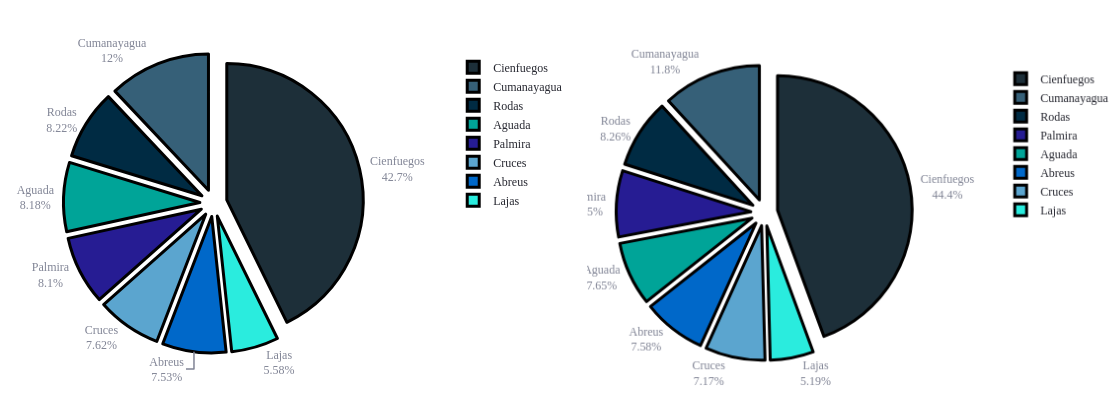
\includegraphics[width=1.0\textwidth]{img/fig1.png}
Se desea partir de analizar la distribución territorial del municipio que se quiere estudiar, por lo que con esta representación \textcolor{blue}{(dividida por edad laboral a la izquierda y edad no laboral a la derecha)} se descubre el predominio de densidad del municipio cabecera con respecto al resto reflejando un claro desblanace de gestión de recursos municipales.

\subsubsection{Educación superior en Cienfuegos}
Siguiendo el devenir de la narrativa expuesta se introduce una observación referente al número de matriculas iniciales y graduados en comparación para cada año en \textcolor{blue}{Cienfuegos} de la educación superior (la cual cabe resaltar que sólo cuenta con 3 universidades y todas en el municipio cabecera)\\\\
Alcanzando a reflejarse el poco volumen de matrículas y la enorme diferencia referente al número de graduados para cada año en una provincia cuyas unicas instituciones de educación superior radican en la cabecera, por lo que claramente las características del entorno para el escenario de quedarse en su provincia natal van esfumando toda idea o interés por seguir en ese sitio.
\begin{center}
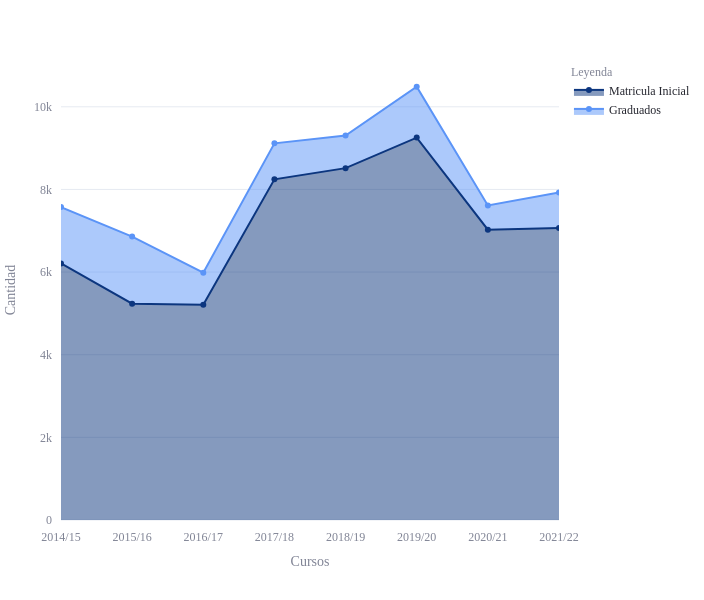
\includegraphics[width=0.7\textwidth]{img/fig2.png}
\end{center}
En medio de esta problemática nace la problemática de la toma de una decisión crucial para la chica, estudiar en la capital lo que quiere o conformarse con lo que su municipio le ofrece, cada alternativa con sus características particulares descritas.\\\\

Luego, acto seguido a introducir al personaje del padre de la joven, con su acción de migrar en el pasado, se procede a analizar los procesos migratorios del territorio cubano, y del municipio en profundidad.
\subsubsection{Procesos migratorios}
Dentro de este apartado se plantea comenzar analizando los movimientos migratorios en la isla por provincias para así evaluar de forma nacional y realizar comparaciones aprovechando la interactividad del recurso presentado en un mapa de densidad desarrollado con el módulo \textcolor{blue}{folium} con el \textcolor{orange}{geojson} anteriormente obtenido.
\subsubsection{Movimientos migratorios}

\begin{center}
    \includegraphics[width=1.0\textwidth]{img/lechee.png}
\end{center}
\begin{itemize}
    \item Predominio del sector no estatal para ambos grupos a partir del 93 para los vacunos y 99 para las cabras, como resultante de la flexibilización de las regulaciones sobre la producción y comercialización de productos lácteos por parte del gobierno cubano, 
    permitiendo a los productores no estatales operar más libremente.
    \item Disminución general vacuna y crecimiento casi constante en cabras. 
\end{itemize}
Sin embargo, el rendimiento anual de vacas de ordeño se mantuvo relativamente semejante en ambos sectores desde 1993, anteriormente se tenían menos libertades para con el rebaño por lo que impería el sector estatal.\\\\
Por otro lado, con respecto a los huevos, su producir tuvo un recorrido general estable y tendiendo al crecimiento hasta la segunda mitad de la segunda década de los años 2000 (exceptuando el período de decrecimiento monstruoso de los 90 por la crisis). Desde ese momento en adelante se ha mantenido oscilando la línea de su desarrollo, principalmente producto de la intensificación del hurto, los sacrificios, la caza y demás factores.
\begin{center}
    \includegraphics[width=1.0\textwidth]{img/11.png}
\end{center}
La producción de carne en general sufrió fue uno de las consecuencias de los valores de existencia y entregas a sacrificio de forma general, siguiendo una línea de disminución por todos los factores influyentes en la isla.
\newpage
\subsubsection{Alimentación}
Acerca de este tema, las fuentes principales de forma general se centraban en los residuos de caña, miel, urea, cachaza, el agua, y la mayor problemática hoy en día, el pienso.
\begin{center}
    \includegraphics[width=1.0\textwidth]{img/1.png}
\end{center}
Para años posteriores a la crisis, con las diferentes relaciones, acuerdos y demás medidas del país se han logrado conseguir algunas fuentes de entrada pero de la misma manera ha subido el valor, por el exceso de demanda de después de la crisis, por lo que la situación 
para los productores no ha sido particularmente sencilla. Y además para despues del 2016 la situación vuelve a decaer producto de intentos del país de diversificar su economía y de complejidades burocráticas con su valor.
\subsubsection{Entidades}
Una de las medidas principales en el campo agrícola fue el surgimiento de la Cooperativa de Crédito y Servicio (CCS) como una herramienta estatal para organizar la producción de los pequeños propietarios rurales y integrarlos activamente en la vida política 
del país. La Asociación Nacional de Agricultores Pequeños (ANAP) jugó un papel crucial en la promoción y apoyo a estas cooperativas. Posteriormente, en el periodo 1975-1985 se expandió la industrialización de la economía cubana, estimulada por la cooperación 
con los países del campo socialista. Como parte de ese proceso, en el Primer Congreso del Partido Comunista de Cuba (PCC) (1975) se planteó como prioridad acelerar el movimiento cooperativo, pero sobre todo encaminarlo a la integración de los campesinos de las 
CCS a lo que se denominó CPA, las cuales socializan los medios de producción, entre ellos la tierra, que deja de ser propiedad privada individual y pasa a ser propiedad colectiva. Tiempo después como contramedida a las repercusiones de la próxima crisis económica de 
1990 se fundan las Unidades Básicas de Producción Cooperativa (UBPC), constituidas en 1993

\clearpage
Desde ese instante se mantuvo dicha estructura hasta el 2011 que surgen las Cooperativas no Agropecuarias para asentarse en el 2013.
\begin{center}
    \includegraphics[width=1.0\textwidth]{img/mapa.png}
\end{center}
Cómo se puede observar en el mapa, la distribución espacial de las instituciones de forma general siempre ha estado concentrada en la capital, y, al excluirla, se aprecia como estas entidades se concentran en mayores cantidades hacia la zona más oriental del país (y Camagüey),
Pinar del Río y Villa Clara en la zona central. Y con una concentración general de un 46,5\%, 35,6\% y 17.1\% de CCS, UBPC y CPA respectivamente para un total de 5688 unidades cooperativas en el año 2012.\\\\

Por otro lado, entrando en un contexto mas contemporaneo, cabe mencionar que las complicaciones y obstaculos (climáticos, epidemiologicas, económicos, etc) que se han ido presentado estos últimos años (sumado a algunos estructurales que se han ido arrastrando desde años atras como la dependencia de importaciones y el impacto 
del bloqueo económico comercial por parte de los Estados Unidos) persisten en la actualidad y se ven reflejadas en todas las carencias de distribución a la poblacion, por parte de la producción, existencia, alimentación del ganado y desarrollo general e institucional. La situación es crítica, pero se puede aprender de la historia
tomando todo este proceso de transición como referencia y antecedente para seguir probando alternativas que nos puedan conducir a un mejor desarrollo como país.

\section{Conclusiones y recomendaciones}
Concluyendo el análisis sobre la ganadería en Cuba, podemos afirmar que el sector enfrenta desafíos significativos pero también oportunidades para su desarrollo. Por un lado, Cuba en algunos momentos ha logrado ciertos avances en la producción de carne y productos lácteos, lo que sugiere una cierta 
resiliencia del sistema agropecuario. Sin embargo, la dependencia de importaciones y el déficit alimentario persisten, que a pesar de presentarse en algún punto de mejoría, se mantienen como problemas estructurales que requieren atención urgente por la situación del deficit general en el sector ganadero cubano.

Para mejorar la situación se recomiendan estrategias de diversificación productiva, inversión en tecnologías y prácticas sostenibles, y fomento del desarrollo rural. Además, es crucial fortalecer las capacidades técnicas y empresariales de los productores, 
así como mejorar la infraestructura agrícola y ganadera. También sería beneficioso revisar y ajustar políticas públicas para alinearlas más estrechamente con las necesidades y posibilidades del sector privado, potenciando su contribución al desarrollo económico y social del país. 
Finalmente, se debe abordar la transición hacia una economía más circular y resiliente, aprovechando recursos locales y reduciendo la dependencia de importaciones, lo cual podría llevar a una mayor autosuficiencia alimentaria y a una industria ganadera más robusta y competitiva.
\end{document}
